\documentclass[10pt]{beamer}
\usepackage{verbatim}
\usepackage[fontset=mac]{ctex}
\usepackage{amsfonts,amsmath,amssymb,mathrsfs}
\usepackage{bm}%希腊字母加粗宏包
%\usetheme{Singapore}%设置演示主题
%\usecolortheme{orchid}%设置颜色主题
\usetheme{Boadilla}
%\usecolortheme{beaver}%设置颜色主题
%\usecolortheme{seagull}
\usepackage[english]{babel}%把英语设为默认语言
\usepackage{pifont}%常规列表环境宏包
\usepackage{verbatim}%多行注释代码
\usepackage{graphicx}%插图
\usepackage{enumerate}
\usepackage{comment}
\usepackage{setspace}
\usepackage{comment}
\setbeamercovered{transparent}

\geometry{left=.8cm,right=.8cm}






\usepackage{marvosym}

\usepackage{tikz}
\usepackage{tikz-3dplot}
\usetikzlibrary{calc, shapes, backgrounds,arrows.meta,patterns}
\usetikzlibrary{decorations.markings,positioning}
\usepackage{xcolor,color}
\def\centerarc[#1](#2)(#3:#4:#5){\draw[#1] ($(#2)+({#5*cos(#3)},{#5*sin(#3)})$) arc (#3:#4:#5);}

%\titlegraphic{\hspace*{9cm}\vspace*{-1cm}\includegraphics[scale=0.2]{school.png}}
\logo{\includegraphics[scale=0.2]{school.png}}

\renewcommand{\baselinestretch}{1.1}

\newcommand{\blue}[1]{{\color{blue} #1}}



\defbeamertemplate{footline}{NGEGFootlineTemplate}{%
	\leavevmode% 离开vmode,也就是离开竖直模式,进入水平模式
	\hbox{%
		\begin{beamercolorbox}[wd=.4\paperwidth,ht=2.25ex,dp=1ex,center]{author in head/foot}%
		\usebeamerfont{author in head/foot}	\ifnum \the\value{page}>0 \insertshortauthor\fi
		\end{beamercolorbox}%
		\begin{beamercolorbox}[wd=.4\paperwidth,ht=2.25ex,dp=1ex,center]{title in head/foot}%
			\ifnum \the\value{page}>0 \usebeamerfont{title in head/foot}\insertshorttitle\fi
		\end{beamercolorbox}%
		\begin{beamercolorbox}[wd=0.2\paperwidth,ht=2.25ex,dp=1ex,center]{date in head/foot}%
			\ifnum \the\value{page}>0 \usebeamerfont{date in head/foot} \insertframenumber{} / \inserttotalframenumber\fi
	\end{beamercolorbox}}%
	%	\vskip0pt%
}
\setbeamertemplate{footline}[NGEGFootlineTemplate]




%\setbeamertemplate{footline}[frame number]%inert page number
%\setbeamertemplate{frametitle}[default][center]
\setbeamerfont{block title}{size=\small}
\setbeamercolor{block title}{use=structure,fg=white,bg=blue!50!black}
\setbeamercolor{block body}{use=structure,fg=black,bg=blue!10!white}

\title[清北师概率 webinar]{ \bf Hydrodynamic Limit for the Facilitated \\Exclusion Process}
\author[Linjie Zhao, Inria Lille Nord Europe]{{\bf Linjie Zhao (赵林杰)}\\
joint work with {\bf Cl{\' e}ment Erignoux} and {\bf Marielle Simon}}

\date{June 2022}

\institute{Inria Lille-Nord Europe, France}

\begin{document}


\begin{frame}
\maketitle
%\begin{table}
%\includegraphics[scale=0.2, right]{school.png}
%\end{table}
\end{frame}

\logo{} 

\section{Introduction}

\begin{frame}
	\tableofcontents[currentsection]
\end{frame}

\begin{frame}

\frametitle{Hydrodynamic Limit}
\begin{itemize}
	\item<1->   In statistical physics, one of the main issues is to establish the partial differential equations that describe the evolution of the thermodynamic characteristics (the temperature, the density, the pressure) of a fluid.
	\item<2->  Example: Hamiltonian systems where particles evolve \blue{deterministically} according to Newton's equations.
	\item<3->  A hard problem due to the Iack of good ergodic properties of the system.
	\item<4-> One of the simplifications is to assume the evolution of the microscopic system to be \blue{stochastic}, \emph{e.g.} stochastic interacting particle systems. See [Liggett'85, 99, Kipnis and Landim'98].  
\end{itemize}
\end{frame}

\begin{frame}{Independent Random Walks}
\begin{table}
	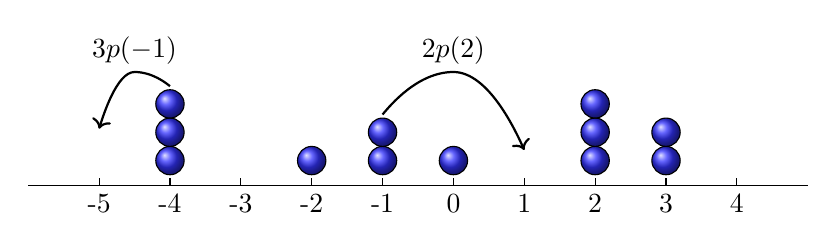
\begin{tikzpicture}[scale=0.9]
		\draw (-2,0) -- (9,0);
		\foreach \x in {-1,0,...,8} 
		\draw  (\x,0) --+(0,0.1);
		\foreach \x/\y in {-1/-5,0/-4,1/-3,2/-2,3/-1,4/0,5/1,6/2,,7/3,8/4}
		\node [below] at (\x,0) {\y};
		
		\foreach \x in {0,2,3,4,6,7}
		\draw[shading=ball,ball color=blue!80] (\x,.35) circle (.2);
		\foreach \x in {0,3,6,7}
		\draw[shading=ball,ball color=blue!80] (\x,.75) circle (.2);
		\foreach \x in {0,6}
		\draw[shading=ball,ball color=blue!80] (\x,1.15) circle (.2);
		\draw[->,thick] (0,1.4) parabola bend (-.5,1.6) (-1,.8);
		\node at (-.5,1.9) {$3p(-1)$};
		\draw[->,thick] (3,1) parabola bend (4,1.6) (5,.5);
		\node at (4,1.9) {$2p(2)$};
%		\node [cross out,draw=red,thick]at (3.5,1.3) {};
%		\node [cross out,draw=red,thick]at (0.5,1.3) {};
%		\draw[<-,thick] (5,.7) parabola bend (5.5,1.3) (6,.7);
%		\node at (5.5,1.5) {$p^\prime>0$};
%		\draw[->,thick] (7,.7) parabola bend (7.5,1.3) (8,.7);
%		\draw[->,thick] (0,.7) parabola bend (.5,1.3) (1,.7);
		%\draw[blue,thick] (-2,-.5)  rectangle (-1,.5) ;
		%\draw[shading=ball,ball color = blue!80] (-1.8,-.3) circle (.2);
		%\draw[shading=ball,ball color = blue!80] (-1.2,-.2) circle (.2);
		%\draw[shading=ball,ball color = blue!80] (-1.5,.2) circle (.2);
		%\draw[->,thick] (-1.5,.7) parabola bend (-.75,1.3) (0,.7);
		%\draw[<-,thick] (-1.5,-.7) parabola bend (-.75,-1.3) (0,-.7);
	\end{tikzpicture}
\end{table}	
\begin{itemize}
\item<1-> For $x \in \mathbb{Z}^d$, let $\eta_x =$ number of particles at site $x$. Let $p(x)$ be a transition probability on $\mathbb{Z}^d$. Particles jump independently  from $x$ to $y$ at rate $p(y-x)$. 
\item<2-> Assume $p(\cdot)$ has \blue{finite range}: $p(x) = 0$ for $|x| >  R$.\\
\blue{Symmetric}: $p(x) = p (-x)$ for all $x \in \mathbb{Z}^d$. \\
\blue{Mean Zero}: $\sum x p(x) = 0$.  \\
\blue{Asymmetric}: $\sum x p(x) \neq 0$.
\end{itemize}
\end{frame}

\begin{frame}{Independent Random Walks}
\begin{itemize}
	\item<1-> For each $N \geq 1$, let $\eta^N$ be a \blue{random} configuration. Let $\rho: \mathbb{R}^d \rightarrow \mathbb{R}_+$ be some \blue{density profile}. We say $\eta^N$ is \blue{associated to the density profile} $\rho$ if for any smooth function $\varphi: \mathbb{R}^d \rightarrow \mathbb{R}$ with compact support, for any $\varepsilon > 0$, 
	\[\lim_{N \rightarrow \infty} P \Big( \Big| \frac{1}{N^d} \sum_{x \in \mathbb{Z}^d} \eta^N_x \varphi \big( \tfrac{x}{N} \big) - \int_{\mathbb{R}^d} \rho(u) \varphi (u) du \Big| > \varepsilon \Big) = 0.\]
	In this case, we denote \blue{$\eta^N \sim \rho(u)$}. Roughly speaking,
	\[\eta^N_x \approx \rho (x/N).\]
	\item<2-> Assume the initial configuration $\eta (0) \sim \rho^{\rm ini}$. Goal: prove for each $t$, $\eta (t\blue{\theta(N)}) \sim \rho(t,u)$. 
	\item<3->  The density profile $\rho(t,u)$ is called the \blue{hydrodynamic equation} of the 
	independent random walks.
\end{itemize}
\end{frame}

\begin{frame}{Independent Random Walks}
\begin{block}{Theorem [Kipnis and Landim'98]}
(i) If $p(\cdot)$ has \blue{mean zero}, then under \blue{diffusive scaling $(\theta(N) = N^2)$}, the hydrodynamic equation is the \blue{heat equation}
\[\begin{cases}
	\partial_{t} \rho (t,u) = \frac{1}{2} \sigma^2 \Delta \rho (t,u),\\
	\rho (0,u) = \rho^{\rm ini} (u),
\end{cases}\]
where $\sigma^2 = \sum x^2 p(x)$.\\
(ii)  If $p(\cdot)$ is \blue{asymmetric}, then under \blue{hyperbolic scaling $(\theta(N) = N)$}, the hydrodynamic equation is the \blue{transport equation}
\[\begin{cases}
	\partial_{t} \rho (t,u) + \frac{1}{2} m \cdot \nabla \rho (t,u) = 0,\\
	\rho (0,u) = \rho^{\rm ini} (u).
\end{cases}\]
where $m = \sum x p(x) \neq 0.$
\end{block}
\end{frame}

\begin{frame}{Macroscopic/Microscopic Mapping}
\begin{itemize}
	\item Symmetric case: diffusive equation
	\begin{table}[]
		\begin{tabular}{l|c|c}
			& Macroscopic             & Microscopic \\ \hline
			Space & $u \approx \frac{x}{N}$ & $x$         \\ \hline
			Time  & $t$                     & $tN^2$     
		\end{tabular}
	\end{table}
CLT: $\frac{S_{N}}{\sqrt{N} }\Rightarrow N(0,1)$.
\item 	Asymmetric case: first order hyperbolic equation
\begin{table}[]
	\begin{tabular}{l|c|c}
		& Macroscopic             & Microscopic \\ \hline
		Space & $u \approx \frac{x}{N}$ & $x$         \\ \hline
		Time  & $t$                     & $tN$     
	\end{tabular}
\end{table}
LLN: $\frac{S_N}{N} \rightarrow \mu$.

\item Sub/super-diffusive scaling.
\end{itemize}
\end{frame}

\begin{frame}{The Stefan Problem}
	
\begin{itemize}
	\item<1-> In one dimension, the Stefan problem reads
	\[\left\{\begin{array}{ll}\partial_{t} \rho=D \partial_{x x}^{2} \rho, & \text { if } 0<x<\Gamma(t), \\ \rho(x, t)=0, & \text { if } x \geqslant \Gamma(t),\end{array} \quad \text { and } \quad \frac{d \Gamma}{d t}=-\partial_{x} \rho(\Gamma(t), t)\right.\]
	\item<2->  {[Gravner and Quastel'00]} for internal DLA\\
	{[Funaki'99]} for ice--water model\\
	{[Blondel, Erignoux, Sasada and Simon'20, B., E. and Simon'21]} for symmetric facilitated exclusion process.
	\item<3-> A new proof for the symmetric case and a new result on the asymmetric case.  
\end{itemize}
\end{frame}

\section{Main Results}

\begin{frame}
	\tableofcontents[currentsection]
\end{frame}

\begin{frame}{Facilitated Exclusion Process}
	
{\onslide<1-> \blue{State space}  $\Sigma_N := \{0,1\}^{\mathbb{L}_N}$, where $\mathbb{L}_N = \mathbb{Z}$ or $\mathbb{T}_N$.   For a  \blue{configuration} $\eta  \in \Sigma_N$, $\eta_x = 1$ if and only if $x$ is occupied by a particle.
\begin{table}
	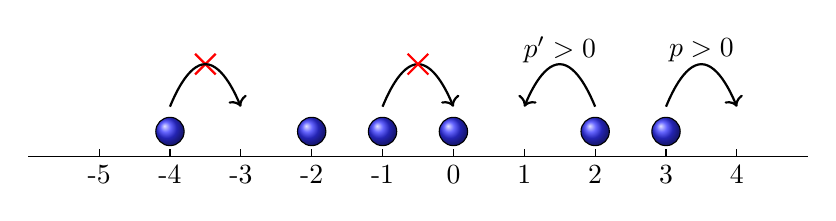
\begin{tikzpicture}[scale=0.9]
		\draw (-2,0) -- (9,0);
		\foreach \x in {-1,0,...,8} 
		\draw  (\x,0) --+(0,0.1);
		\foreach \x/\y in {-1/-5,0/-4,1/-3,2/-2,3/-1,4/0,5/1,6/2,,7/3,8/4}
		\node [below] at (\x,0) {\y};
		
		\foreach \x in {0,2,3,4,6,7}
		\draw[shading=ball,ball color=blue!80] (\x,.35) circle (.2);
		\draw[->,thick] (3,.7) parabola bend (3.5,1.3) (4,.7);
		\node [cross out,draw=red,thick]at (3.5,1.3) {};
		\node [cross out,draw=red,thick]at (0.5,1.3) {};
		\draw[<-,thick] (5,.7) parabola bend (5.5,1.3) (6,.7);
		\node at (5.5,1.5) {$p^\prime>0$};
		\draw[->,thick] (7,.7) parabola bend (7.5,1.3) (8,.7);
		\node at (7.5,1.5) {$p>0$};
		\draw[->,thick] (0,.7) parabola bend (.5,1.3) (1,.7);
		%\draw[blue,thick] (-2,-.5)  rectangle (-1,.5) ;
		%\draw[shading=ball,ball color = blue!80] (-1.8,-.3) circle (.2);
		%\draw[shading=ball,ball color = blue!80] (-1.2,-.2) circle (.2);
		%\draw[shading=ball,ball color = blue!80] (-1.5,.2) circle (.2);
		%\draw[->,thick] (-1.5,.7) parabola bend (-.75,1.3) (0,.7);
		%\draw[<-,thick] (-1.5,-.7) parabola bend (-.75,-1.3) (0,-.7);
	\end{tikzpicture}
\end{table}	
}

\begin{itemize}
	\item<2->  \blue{Exclusion} rule: there is at most one particle at each site.
	\item<3-> \blue{Facilitated} rule: a particle has to be pushed forward in order to jump.
	\item<4-> \blue{Symmetric}: $p = p^\prime$, $\mathbb{L}_N = \mathbb{T}_N$. \blue{Asymmetric}: $p > p^\prime$, $\mathbb{L}_N = \mathbb{Z}$.
\end{itemize}
\end{frame}

\begin{frame}{Facilitated Exclusion Process}
	
	\begin{itemize}
		\item<1-> For $x,y \in \mathbb{L}_N$, $\eta^{x,y}$denotes the configuration obtained from $\eta$ by swapping the values at sites $x$ and $y$.
		\item<2-> The \blue{jump rate} is given by
		\[c_{x, x+1}(\eta)=p \eta_{x-1} \eta_{x}\left(1-\eta_{x+1}\right)+p^{\prime}\left(1-\eta_{x}\right) \eta_{x+1} \eta_{x+2}.\]
		\begin{table}
			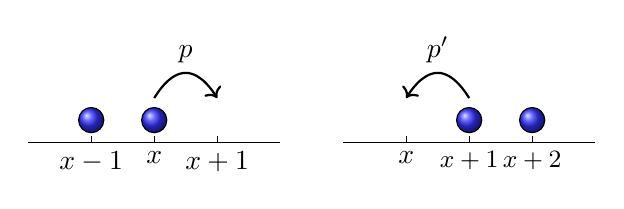
\begin{tikzpicture}[scale=0.8]
				\draw (-1,0) -- (3,0);
				\foreach \x in {0,1,2} 
				\draw  (\x,0) --+(0,0.1);
				\node [below] at (0,0) {$x-1$};
				\node [below] at (1,0) {$x$};
				\node [below] at (2,0) {$x+1$};
				\foreach \x in {0,1}
				\draw[shading=ball,ball color=blue!80] (\x,.35) circle (.2);
				\draw[->,thick] (1,.7) parabola bend (1.5,1.1) (2,.7);
				\node[above] at (1.5,1.1) {$p$};
				
				\draw (4,0) -- (8,0);
				\foreach \x in {5,6,7} 
				\draw  (\x,0) --+(0,0.1);
				\node [below] at (5,0) {$x$};
				\node [below] at (6,0) {\small $x+1$};
				\node [below] at (7,0) {\small $x+2$};
				\foreach \x in {6,7}
				\draw[shading=ball,ball color=blue!80] (\x,.35) circle (.2);
				\draw[->,thick] (6,.7) parabola bend (5.5,1.1) (5,.7);
				\node[above] at (5.5,1.1) {$p^\prime$};
				%\draw[blue,thick] (-2,-.5)  rectangle (-1,.5) ;
				%\draw[shading=ball,ball color = blue!80] (-1.8,-.3) circle (.2);
				%\draw[shading=ball,ball color = blue!80] (-1.2,-.2) circle (.2);
				%\draw[shading=ball,ball color = blue!80] (-1.5,.2) circle (.2);
				%\draw[->,thick] (-1.5,.7) parabola bend (-.75,1.3) (0,.7);
				%\draw[<-,thick] (-1.5,-.7) parabola bend (-.75,-1.3) (0,-.7);
			\end{tikzpicture}
		\end{table}	
		\item<3-> For any local function $f: \Sigma_N \rightarrow \mathbb{R}$, the \blue{infinitesimal generator} is
		\[\mathscr{L}_{N}^{\mathrm{FEX}} f(\eta):=\sum_{x \in \mathbb{L}_{N}} c_{x, x+1}(\eta)\left(f\left(\eta^{x, x+1}\right)-f(\eta)\right).\]
	\end{itemize}
\end{frame}

\begin{frame}{Phase Transitions}
	
{\onslide<1-> The process displays a \blue{phase transition} at the critical particle density \blue{$\rho_c = 1/2$}.}
\begin{itemize}
	\item<2-> If initially $\rho > 1/2$, then the system evolves until there are no longer two neighboring empty sites.
	\begin{table}
		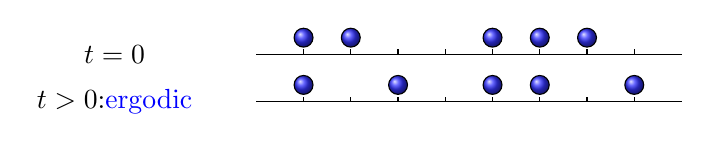
\begin{tikzpicture}[scale=0.6]
			\node at (-5,0) {$t=0$};
			\draw (-2,0) -- (7,0);
			\foreach \x in {-1,0,...,5,6} 
			\draw  (\x,0) -- +(0,0.1);
%			\foreach \x/\y in {-1/-5,0/-4,1/-3,2/-2,3/-1,4/0,5/1,6/2,,7/3,8/4}
%			\node [below] at (\x,0) {\y};
			
			\foreach \x in {-1,0,3,4,5}
			\draw[shading=ball,ball color=blue!80] (\x,.35) circle (.2);
%			\draw[->,thick] (3,.7) parabola bend (3.5,1.3) (4,.7);
%			\node [cross out,draw=red,thick]at (3.5,1.3) {};
%			\node [cross out,draw=red,thick]at (0.5,1.3) {};
%			\draw[<-,thick] (5,.7) parabola bend (5.5,1.3) (6,.7);
%			\node at (5.5,1.5) {$p^\prime>0$};
%			\draw[->,thick] (7,.7) parabola bend (7.5,1.3) (8,.7);
%			\node at (7.5,1.5) {$p>0$};
%			\draw[->,thick] (0,.7) parabola bend (.5,1.3) (1,.7);
			%\draw[blue,thick] (-2,-.5)  rectangle (-1,.5) ;
			%\draw[shading=ball,ball color = blue!80] (-1.8,-.3) circle (.2);
			%\draw[shading=ball,ball color = blue!80] (-1.2,-.2) circle (.2);
			%\draw[shading=ball,ball color = blue!80] (-1.5,.2) circle (.2);
			%\draw[->,thick] (-1.5,.7) parabola bend (-.75,1.3) (0,.7);
			%\draw[<-,thick] (-1.5,-.7) parabola bend (-.75,-1.3) (0,-.7);
			\node at (-5,-1) {$t>0$:\blue{ergodic}};
			\draw (-2,-1) -- (7,-1);
			\foreach \x in {-1,0,...,5,6} 
			\draw  (\x,-1) -- +(0,0.1);
			%			\foreach \x/\y in {-1/-5,0/-4,1/-3,2/-2,3/-1,4/0,5/1,6/2,,7/3,8/4}
			%			\node [below] at (\x,0) {\y};
			
			\foreach \x in {-1,1,3,4,6}
			\draw[shading=ball,ball color=blue!80] (\x,-0.65) circle (.2);
		\end{tikzpicture}
	\end{table}	
	
	\item<3-> If initially $\rho < 1/2$, then the system evolves until all particles are isolated, and thus can no longer move.
		\begin{table}
		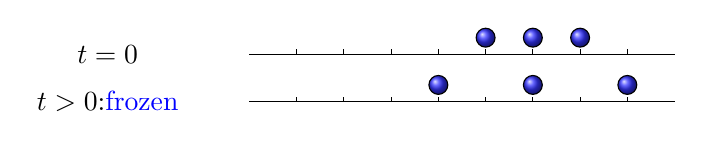
\begin{tikzpicture}[scale=0.6]
			\node at (-5,0) {$t=0$};
			\draw (-2,0) -- (7,0);
			\foreach \x in {-1,0,...,5,6} 
			\draw  (\x,0) -- +(0,0.1);
			%			\foreach \x/\y in {-1/-5,0/-4,1/-3,2/-2,3/-1,4/0,5/1,6/2,,7/3,8/4}
			%			\node [below] at (\x,0) {\y};
			
			\foreach \x in {3,4,5}
			\draw[shading=ball,ball color=blue!80] (\x,.35) circle (.2);
			%			\draw[->,thick] (3,.7) parabola bend (3.5,1.3) (4,.7);
			%			\node [cross out,draw=red,thick]at (3.5,1.3) {};
			%			\node [cross out,draw=red,thick]at (0.5,1.3) {};
			%			\draw[<-,thick] (5,.7) parabola bend (5.5,1.3) (6,.7);
			%			\node at (5.5,1.5) {$p^\prime>0$};
			%			\draw[->,thick] (7,.7) parabola bend (7.5,1.3) (8,.7);
			%			\node at (7.5,1.5) {$p>0$};
			%			\draw[->,thick] (0,.7) parabola bend (.5,1.3) (1,.7);
			%\draw[blue,thick] (-2,-.5)  rectangle (-1,.5) ;
			%\draw[shading=ball,ball color = blue!80] (-1.8,-.3) circle (.2);
			%\draw[shading=ball,ball color = blue!80] (-1.2,-.2) circle (.2);
			%\draw[shading=ball,ball color = blue!80] (-1.5,.2) circle (.2);
			%\draw[->,thick] (-1.5,.7) parabola bend (-.75,1.3) (0,.7);
			%\draw[<-,thick] (-1.5,-.7) parabola bend (-.75,-1.3) (0,-.7);
			\node at (-5,-1) {$t>0$:\blue{frozen}};
			\draw (-2,-1) -- (7,-1);
			\foreach \x in {-1,0,...,5,6} 
			\draw  (\x,-1) -- +(0,0.1);
			%			\foreach \x/\y in {-1/-5,0/-4,1/-3,2/-2,3/-1,4/0,5/1,6/2,,7/3,8/4}
			%			\node [below] at (\x,0) {\y};
			
			\foreach \x in {2,4,6}
			\draw[shading=ball,ball color=blue!80] (\x,-0.65) circle (.2);
		\end{tikzpicture}
		\end{table}
\end{itemize}
\end{frame}

\begin{frame}{Invariant Measures on $\{0,1\}^\mathbb{Z}$}
	\small 
\begin{itemize}
\item<1-> For each $\rho > 1/2$, the process has a translation invariant and invariant measure $\pi_{\rho}$, which is \blue{not} product. (\blue{exponentially decay})
\[\ldots 01110101101\ldots\]
\item<2-> Put a hole in some position with probability $1-\rho$, then put a random \blue{geometric number} of parameter $\frac{1-\rho}{\rho}$ particles to its right, then a hole, starts again and so on. 
	\begin{align*} 	\pi_\rho (11) &= \pi_\rho (1) - \pi_{\rho} (01) = \rho - (1-\rho) \times 1 = 2 \rho -1.\\
	\pi_\rho (111) &= \pi_\rho (11) - \pi_{\rho} (011) \\
	&= (2\rho-1) - (1-\rho) \times 1 \times \frac{2\rho-1}{\rho} = \frac{(2\rho-1)^2}{\rho}.
\end{align*}
\item<3-> For $\rho \leq 1/2$, $\pi_\rho$ is concentrated on frozen configurations.
\[\rho = 1/3 \qquad \ldots 001001001001001 \ldots\]
\end{itemize}
\end{frame}

\begin{frame}{Facilitated Exclusion Process}
\begin{itemize}
	\item A new universality class (critical density, critical exponents) in the physics literature.
	\item Belongs to KPZ universality class [Baik, Barraquand, Corwin and Suidan'16].
	\item Stationary states of the model, see the work of Goldstein, Lebowitz, Speer etc. and [Chen and Z.'19].
	\item Open in higher dimensions.
\end{itemize}
\end{frame}

\begin{frame}{Hydrodynamic Limit}
\begin{block}{Theorem  [Blondel \emph{et al.} '20, '21, Erignoux, Simon and Z. '22]}
(i) In the symmetric case $p=p^\prime =1$, under \blue{diffusive scaling}, the hydrodynamic equation is given by
\[\partial_t \rho  (t,u)= \partial_u^2 \Big( \frac{2\rho(t,u)-1}{\rho (t,u)}  \blue{\mathbf{1}_{\{\rho(t,u) > 1/2}\}} \Big) \] 
with initial condition $\rho^{\rm ini}$. \blue{(weak solution, uniqueness since $\frac{2\rho-1}{\rho} \mathbf{1}_{\rho > 1/2}$ is nondecreasing)}	\\
(ii) In the asymmetric case, under \blue{hyperbolic scaling}, the hydrodynamic equation is given by
\[	\partial_t \rho (t,u)  + (p-p^{\prime}) \partial_u \Big( \frac{(1-\rho(t,u))(2\rho(t,u)-1)}{\rho (t,u) }  \blue{\mathbf{1}_{\{\rho (t,u)> 1/2\}}} \Big) = 0\]
with initial condition $\rho^{\rm ini}$.	\blue{(entropy solution)}
\end{block}
\end{frame}





\begin{frame}{Entropy solution [Serre'99]}
\onslide<1->{Consider 
\begin{equation*}
\begin{cases}
	\partial_t \rho (t,u) + \partial_u f\,(\rho(t,u)) = 0, \quad u \in \mathbb{R}, t > 0,\\
	\rho (0,u) = \rho^{\rm ini} (u), \quad u \in \mathbb{R}.
\end{cases}
\end{equation*}
The weak solution is not unique!  Let $(E,F)$ be an \blue{entropy-entropy-flux  pair}, i.e. $E^{\,\prime} f^{\,\prime} = F^{\prime}$. Formally,
\[\partial_t E(\rho(t,u)) + \partial_u F(\rho(t,u)) = 0.\]}
\onslide<2->{(Entropy inequality)  For any $E$ convex,
\[\partial_t E(\rho(t,u)) + \partial_u F(\rho(t,u)) \leq  0\]
in the sense of distributions.\\}
\onslide<3->{The entropy solution could be obtained as $\lim_{\varepsilon \rightarrow 0} \rho^{\varepsilon}$, where
\[\partial_t \rho^\varepsilon (t,u) + \partial_u f\,(\rho^\varepsilon(t,u)) = \varepsilon \partial_u^2 \rho^\varepsilon (t,u).\]}
\end{frame}



\section{Formal Proof}

\begin{frame}
	\tableofcontents[currentsection]
\end{frame}

\begin{frame}{$p=p^\prime =1$}
	
	\begin{itemize}
		\item<1-> First recall
		\[\rho (t,\tfrac{x}{N}) \approx \mathbb{E} [\eta_x (\blue{tN^2})], \quad x \in \mathbb{T}_N,\]
		or equivalently,
		\[\rho (t,u) \approx \mathbb{E} [\eta_{uN} (tN^2)], \quad u \in \mathbb{T}.\]
		
		\item<2-> Conservation law
		\[\frac{d}{dt} \mathbb{E} [\eta_{uN} (tN^2)] = N^2 \Big( \mathbb{E} [\,j_{uN-1,uN} (tN^2)] -  \mathbb{E} [\,j_{uN,uN+1} (tN^2)] \Big),\]
		where $j_{x,x+1} (t)$ is the instantaneous current from $x$ to $x+1$,
		\[j_{x,x+1} (t) = \eta_{x-1}(t) \eta_{x}(t) (1 - \eta_{x+1} (t)) -  \eta_{x+2}(t) \eta_{x+1}(t) (1 - \eta_{x} (t)).\]
	\end{itemize}
\end{frame}

\begin{frame}{$p=p^\prime =1$}
	
	\begin{itemize}
		\item<1-> \blue{Gradient condition}
		\begin{align*}
		j_{x,x+1} (t) &= \eta_{x-1}(t) \eta_{x}(t) (1 - \eta_{x+1} (t)) -  \eta_{x+2}(t) \eta_{x+1}(t) (1 - \eta_{x} (t))\\
&= h_x (t) - h_{x+1} (t),
		\end{align*}
	where
	\[h_x (t) =\eta_{x-1} (t) \eta_x (t)+\eta_x (t) \eta_{x+1} (t)-\eta_{x-1} (t) \eta_{x} (t)\eta_{x+1} (t).\]

	
	\item<2-> Therefore,
	\[\partial_t \rho (t,u) \approx N^2 \Big( \mathbb{E} [h_{uN-1} (tN^2)] +  \mathbb{E} [h_{uN+1} (tN^2)] - 2  \mathbb{E} [h_{uN} (tN^2)] \Big).  \]
	Remark: Most of the models are non-gradient and are more difficult!
	\end{itemize}

\end{frame}

\begin{frame}{$p=p^\prime =1$}
	\begin{itemize}
		\item<1-> \blue{Local ergodicity}: the distribution of the process at time $tN^2$ around site $uN$ is approximately $\pi_{\rho (t,u)}$. (\blue{replacement lemmas})
		
		\item<2-> For $\rho (t,u)> 1/2$,
		\begin{align*}
			\mathbb{E} [h_{uN} (tN^2)] &\approx \pi_{\rho (t,u)} (h) = 2 \pi_{\rho (t,u)} (11) - \pi_{\rho (t,u)} (111)\\
			&= \frac{2 \rho(t,u) - 1}{\rho(t,u)}.
		\end{align*}
	The above term is zero if $\rho (t,u) \leq 1/2$. 
	\item<3-> Let $\mathcal{H}(\rho) = \frac{2 \rho-1}{\rho} \mathbf{1}_{\rho > 1/2}$. Then,
	\begin{align*}
		\partial_t \rho (t,u) &\approx N^2  \Big( \mathcal{H}(\rho(t,u - \tfrac{1}{N})) + \mathcal{H}(\rho(t,u + \tfrac{1}{N})) - 2 \mathcal{H}(\rho(t,u )) \Big) \\
		&\approx \partial_u^2 \mathcal{H}(\rho(t,u)).
	\end{align*}
	\end{itemize}
\end{frame}

\begin{frame}{General methods [Kipnis and Landim'99]}
\begin{itemize}
	\item<1->  Entropy (GPV) method: uniqueness of solutions, explicit invariant measures.
	\item<2-> Yau's relative entropy method:  smoothness of solutions. (Shocks in hyperbolic systems.)
	\item<3-> Attractiveness method [Rezakhanlou'91]. 
	\item<4-> Compensated compactness method [Fritz'04]: Log-Sobolev inequality (a hard problem).
\end{itemize}
\end{frame}

\section{Mapping}

\begin{frame}
	\tableofcontents[currentsection]
\end{frame}

\begin{frame}{Mapping}

\begin{itemize}
	
	\item<1-> Label the empty sites from the left to the right in an increasing order.
	Let $X_y (t)$ be the position of the $y$--th empty site at time $t$.
	\begin{table}
		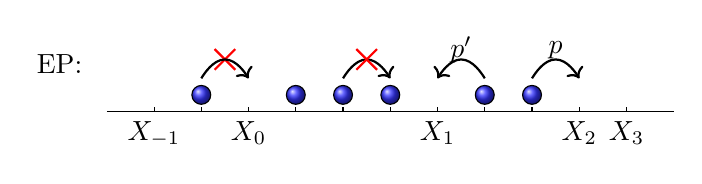
\begin{tikzpicture}[scale=0.6]
			\node at (-3,1) {EP:};
			\draw (-2,0) -- (10,0);
			\foreach \x in {-1,0,...,8,9} 
			\draw  (\x,0) --+(0,0.1);
			%		\foreach \x/\y in {-1/-5,0/-4,1/-3,2/-2,3/-1,4/0,5/1,6/2,,7/3,8/4}
			%		\node [below] at (\x,0) {\y};
			\foreach \x/\y in {-1/-1,1/0,5/1,8/2,9/3}
			\node [below] at (\x,0) {$X_{\y} $};
			
			\foreach \x in {0,2,3,4,6,7}
			\draw[shading=ball,ball color=blue!80] (\x,.35) circle (.2);
			\draw[->,thick] (3,.7) parabola bend (3.5,1.1) (4,.7);
			\node [cross out,draw=red,thick]at (3.5,1.1) {};
			\node [cross out,draw=red,thick]at (0.5,1.1) {};
			\draw[<-,thick] (5,.7) parabola bend (5.5,1.1) (6,.7);
			\node at (5.5,1.3) {$p^\prime$};
			\draw[->,thick] (7,.7) parabola bend (7.5,1.1) (8,.7);
			\node at (7.5,1.3) {$p$};
			\draw[->,thick] (0,.7) parabola bend (.5,1.1) (1,.7);
			%\draw[blue,thick] (-2,-.5)  rectangle (-1,.5) ;
			%\draw[shading=ball,ball color = blue!80] (-1.8,-.3) circle (.2);
			%\draw[shading=ball,ball color = blue!80] (-1.2,-.2) circle (.2);
			%\draw[shading=ball,ball color = blue!80] (-1.5,.2) circle (.2);
			%\draw[->,thick] (-1.5,.7) parabola bend (-.75,1.3) (0,.7);
			%\draw[<-,thick] (-1.5,-.7) parabola bend (-.75,-1.3) (0,-.7);
		\end{tikzpicture}
	\end{table}	
	\item<2-> Let $\omega_y (t)\in \{0,1,2,\ldots\}$ be the number of particles between the $y$--th and $(y+1)$--th empty sites at time $t$.
	\begin{table}
		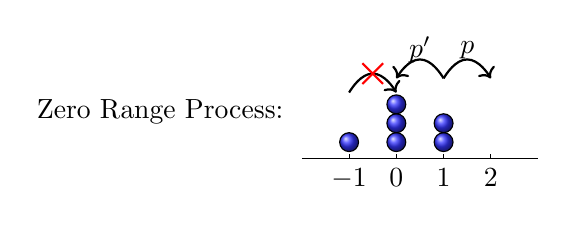
\begin{tikzpicture}[scale=0.6]
			\node at (-2,1) {Zero Range Process:};
			\draw (1,0)--(6,0);
			\foreach \x in {2,3,4,5} 
			\draw  (\x,0) --+(0,0.1);
			\foreach \x/\y in {-1/2,0/3,1/4,2/5} 
			\node[below] at (\y,0) {$\x$};
			\foreach \x in {2,3,4}
			\draw[shading=ball,ball color=blue!80] (\x,.35) circle (.2);
			\draw[shading=ball,ball color=blue!80] (3,.75) circle (.2);
			\draw[shading=ball,ball color=blue!80] (3,1.15) circle (.2);
			\draw[shading=ball,ball color=blue!80] (4,.75) circle (.2);
			\draw[->,thick] (4,1.7) parabola bend (4.5,2.1) (5,1.7);
			\draw[->,thick] (2,1.4) parabola bend (2.5,1.8) (3,1.4);
			\node [cross out,draw=red,thick]at (2.5,1.8) {};
			\node at (4.5,2.3) {$p$};
			\draw[->,thick] (4,1.7) parabola bend (3.5,2.1) (3,1.7);
			\node at (3.5,2.3) {$p^\prime$};
		\end{tikzpicture}
	\end{table}	
\item<3-> A particle jumps to its right (resp. left) at rate $p \mathbf{1}_{\omega_y \geq 2}$ (resp. $p^{\,\prime} \mathbf{1}_{\omega_y \geq 2}$). 
\end{itemize}
\end{frame}

\begin{frame}{Mapping}

Recall $\alpha (t,v)$: density profile for ZRP, $\rho (t,u)$ for EP.
\[\rho (t,u) = \frac{\alpha (t,v)}{1+ \alpha(t,v)}, \quad \alpha (t,v) = \frac{\rho(t,u)}{1-\rho (t,u)}.\] 
	\begin{table}
	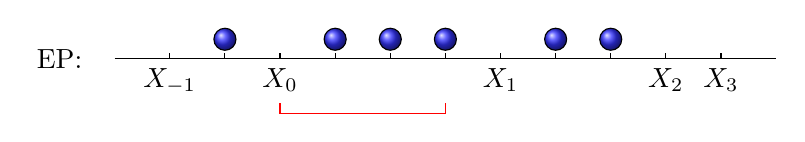
\begin{tikzpicture}[scale=0.7]
		\node at (-3,0) {EP:};
		\draw (-2,0) -- (10,0);
		\foreach \x in {-1,0,...,8,9} 
		\draw  (\x,0) --+(0,0.1);
		%		\foreach \x/\y in {-1/-5,0/-4,1/-3,2/-2,3/-1,4/0,5/1,6/2,,7/3,8/4}
		%		\node [below] at (\x,0) {\y};
		\foreach \x/\y in {-1/-1,1/0,5/1,8/2,9/3}
		\node [below] at (\x,0) {$X_{\y} $};
		\draw[-,color=red]  (1,-1)--(4,-1);
		\draw[color=red] (1,-1)--(1,-.8);
		\draw[color=red] (4,-1)--(4,-.8);
		
		
	\foreach \x in {0,2,3,4,6,7}
	\draw[shading=ball,ball color=blue!80] (\x,.35) circle (.2);
%		\draw[->,thick] (3,.7) parabola bend (3.5,1.1) (4,.7);
%		\node [cross out,draw=red,thick]at (3.5,1.1) {};
%		\node [cross out,draw=red,thick]at (0.5,1.1) {};
%		\draw[<-,thick] (5,.7) parabola bend (5.5,1.1) (6,.7);
%		\node at (5.5,1.3) {$p^\prime$};
%		\draw[->,thick] (7,.7) parabola bend (7.5,1.1) (8,.7);
%		\node at (7.5,1.3) {$p$};
		%\draw[->,thick] (0,.7) parabola bend (.5,1.1) (1,.7);
		%\draw[blue,thick] (-2,-.5)  rectangle (-1,.5) ;
		%\draw[shading=ball,ball color = blue!80] (-1.8,-.3) circle (.2);
		%\draw[shading=ball,ball color = blue!80] (-1.2,-.2) circle (.2);
		%\draw[shading=ball,ball color = blue!80] (-1.5,.2) circle (.2);
		%\draw[->,thick] (-1.5,.7) parabola bend (-.75,1.3) (0,.7);
		%\draw[<-,thick] (-1.5,-.7) parabola bend (-.75,-1.3) (0,-.7);
	\end{tikzpicture}
\end{table}	
	\begin{table}
	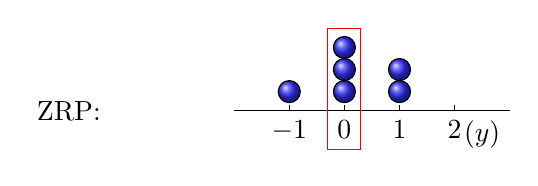
\begin{tikzpicture}[scale=0.7]
		\node at (-2,0) {ZRP:};
		\draw (1,0)--(6,0);
		\foreach \x in {2,3,4,5} 
		\draw  (\x,0) --+(0,0.1);
		\foreach \x/\y in {-1/2,0/3,1/4,2/5} 
		\node[below] at (\y,0) {$\x$};
		\foreach \x in {2,3,4}
		\draw[shading=ball,ball color=blue!80] (\x,.35) circle (.2);
		\draw[shading=ball,ball color=blue!80] (3,.75) circle (.2);
		\draw[shading=ball,ball color=blue!80] (3,1.15) circle (.2);
		\draw[shading=ball,ball color=blue!80] (4,.75) circle (.2);
		\node[below] at (5.5,0) {$(y)$};
		\draw[color=red] (2.7,-.7) rectangle (3.3,1.5);
%		\draw[->,thick] (4,1.7) parabola bend (4.5,2.1) (5,1.7);
%		\draw[->,thick] (2,1.4) parabola bend (2.5,1.8) (3,1.4);
%		\node [cross out,draw=red,thick]at (2.5,1.8) {};
%		\node at (4.5,2.3) {$p$};
%		\draw[->,thick] (4,1.7) parabola bend (3.5,2.1) (3,1.7);
%		\node at (3.5,2.3) {$p^\prime$};
	\end{tikzpicture}
\end{table}	

\end{frame}

\begin{frame}{Mapping}
Relation between $u = u(t,v)$ and $v = v(t,u)$: $x,u$ for EP, $y,v$ for ZRP.
\[x = X_0 (t)+ \sum_{y^{\,\prime} = 0}^{y} [1+\omega_{y^{\,\prime}} (t)] \quad \Rightarrow \quad u = v_0(t) + \int_0^{v} [1+\alpha(t,v^{\,\prime})] dv^{\,\prime}.\]
\[y = \sum_{x^{\,\prime}=X_0(t)}^{x} [1-\eta_{x^{\,\prime}} (t)] \quad \Rightarrow \quad v = \int_{v_0 (t)}^{u} [1-\rho(t,u^{\,\prime})] du.\]
\begin{table}
	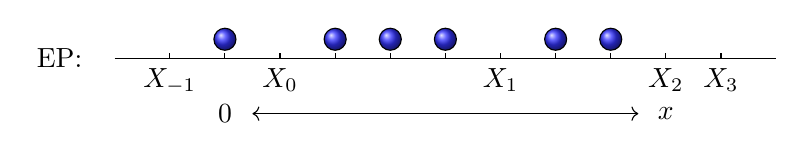
\begin{tikzpicture}[scale=0.7]
		\node at (-3,0) {EP:};
		\draw (-2,0) -- (10,0);
		\foreach \x in {-1,0,...,8,9} 
		\draw  (\x,0) --+(0,0.1);
		%		\foreach \x/\y in {-1/-5,0/-4,1/-3,2/-2,3/-1,4/0,5/1,6/2,,7/3,8/4}
		%		\node [below] at (\x,0) {\y};
		\foreach \x/\y in {-1/-1,1/0,5/1,8/2,9/3}
		\node [below] at (\x,0) {$X_{\y} $};
		\node  at (0,-1) {$0$};
		\node  at (8,-1) {$x$};
		\draw[<->]  (0.5,-1)--(7.5,-1);
		
		
		\foreach \x in {0,2,3,4,6,7}
		\draw[shading=ball,ball color=blue!80] (\x,.35) circle (.2);
		%		\draw[->,thick] (3,.7) parabola bend (3.5,1.1) (4,.7);
		%		\node [cross out,draw=red,thick]at (3.5,1.1) {};
		%		\node [cross out,draw=red,thick]at (0.5,1.1) {};
		%		\draw[<-,thick] (5,.7) parabola bend (5.5,1.1) (6,.7);
		%		\node at (5.5,1.3) {$p^\prime$};
		%		\draw[->,thick] (7,.7) parabola bend (7.5,1.1) (8,.7);
		%		\node at (7.5,1.3) {$p$};
		%\draw[->,thick] (0,.7) parabola bend (.5,1.1) (1,.7);
		%\draw[blue,thick] (-2,-.5)  rectangle (-1,.5) ;
		%\draw[shading=ball,ball color = blue!80] (-1.8,-.3) circle (.2);
		%\draw[shading=ball,ball color = blue!80] (-1.2,-.2) circle (.2);
		%\draw[shading=ball,ball color = blue!80] (-1.5,.2) circle (.2);
		%\draw[->,thick] (-1.5,.7) parabola bend (-.75,1.3) (0,.7);
		%\draw[<-,thick] (-1.5,-.7) parabola bend (-.75,-1.3) (0,-.7);
	\end{tikzpicture}
\end{table}	
\begin{table}
	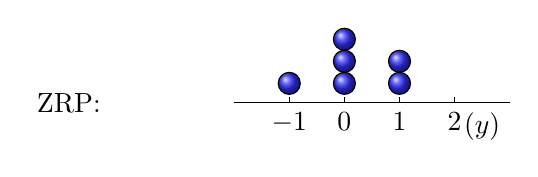
\begin{tikzpicture}[scale=0.7]
		\node at (-2,0) {ZRP:};
		\draw (1,0)--(6,0);
		\foreach \x in {2,3,4,5} 
		\draw  (\x,0) --+(0,0.1);
		\foreach \x/\y in {-1/2,0/3,1/4,2/5} 
		\node[below] at (\y,0) {$\x$};
		\foreach \x in {2,3,4}
		\draw[shading=ball,ball color=blue!80] (\x,.35) circle (.2);
		\draw[shading=ball,ball color=blue!80] (3,.75) circle (.2);
		\draw[shading=ball,ball color=blue!80] (3,1.15) circle (.2);
		\draw[shading=ball,ball color=blue!80] (4,.75) circle (.2);
		\node[below] at (5.5,0) {$(y)$};
		%		\draw[->,thick] (4,1.7) parabola bend (4.5,2.1) (5,1.7);
		%		\draw[->,thick] (2,1.4) parabola bend (2.5,1.8) (3,1.4);
		%		\node [cross out,draw=red,thick]at (2.5,1.8) {};
		%		\node at (4.5,2.3) {$p$};
		%		\draw[->,thick] (4,1.7) parabola bend (3.5,2.1) (3,1.7);
		%		\node at (3.5,2.3) {$p^\prime$};
	\end{tikzpicture}
\end{table}
\end{frame}


\begin{frame}{Facilitated Zero Range Process}
	
	\begin{itemize}
		\item<1-> If there are at least two particles at a site, then one of them jumps to the right (resp. to the left) at rate $p$ (resp. $p^\prime$).
		\begin{table}
			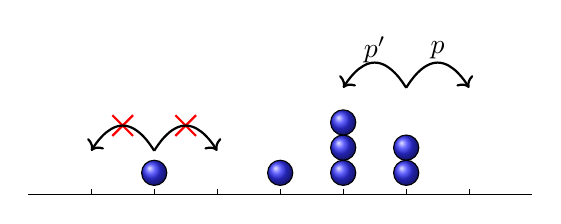
\begin{tikzpicture}[scale=0.8]
				\draw (-2,0)--(6,0);
				\foreach \x in {-1,0,1,2,3,4,5} 
				\draw  (\x,0) --+(0,0.1);
				%		\foreach \x/\y in {-1/2,0/3,1/4,2/5} 
				%		\node[below] at (\y,0) {$\x$};
				\foreach \x in {0,2,3,4}
				\draw[shading=ball,ball color=blue!80] (\x,.35) circle (.2);
				\draw[shading=ball,ball color=blue!80] (3,.75) circle (.2);
				\draw[shading=ball,ball color=blue!80] (3,1.15) circle (.2);
				\draw[shading=ball,ball color=blue!80] (4,.75) circle (.2);
				\draw[->,thick] (4,1.7) parabola bend (4.5,2.1) (5,1.7);
				\node at (4.5,2.3) {$p$};
				\draw[->,thick] (4,1.7) parabola bend (3.5,2.1) (3,1.7);
				\node at (3.5,2.3) {$p^\prime$};
				\node [cross out,draw=red,thick]at (0.5,1.1) {};
				\node [cross out,draw=red,thick]at (-0.5,1.1) {};
				\draw[->,thick] (0,0.7) parabola bend (.5,1.1) (1,.7);
				\draw[->,thick] (0,0.7) parabola bend (-0.5,1.1) (-1,.7);
			\end{tikzpicture}
		\end{table}	
		\item<2-> The critical particle density is $\alpha_c = 1$.
		\item<3->  The process has a family of \blue{product} invariant measures when the particle density $\alpha > 1$.
		\item<4-> The process is \blue{attractive}.
	\end{itemize}
\end{frame}

\begin{frame}{Attractiveness}

{\onslide<1-> Attractiveness: if $\omega_y (0) \leq \widetilde{\omega}_y (0)$ for all $y$, then there exists a coupling such that $\omega_y (t) \leq \widetilde{\omega}_y (t)$ for all $y$ and $t > 0$.}
\onslide<2->{\begin{table}
	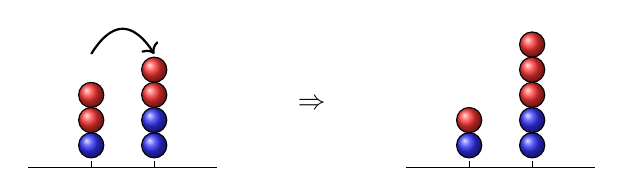
\begin{tikzpicture}[scale=0.8]
		\draw (-2,0)--(1,0);
		\foreach \x in {-1,0} 
		\draw  (\x,0) --+(0,0.1);
		%		\foreach \x/\y in {-1/2,0/3,1/4,2/5} 
		%		\node[below] at (\y,0) {$\x$};
		\foreach \x in {0,-1}
		\draw[shading=ball,ball color=blue!80] (\x,.35) circle (.2);
		\draw[shading=ball,ball color=blue!80] (0,.75) circle (.2);
		\draw[shading=ball,ball color=red!80] (0,1.15) circle (.2);
		\draw[shading=ball,ball color=red!80] (0,1.55) circle (.2);
		\draw[shading=ball,ball color=red!80] (-1,1.15) circle (.2);
		\draw[shading=ball,ball color=red!80] (-1,.75) circle (.2);
		\draw[->,thick] (-1,1.8) parabola bend (-0.5,2.2) (0,1.8);
			\node at (2.5,1) {$\Rightarrow$};
%		\node at (4.5,2.3) {$p$};
%		\draw[->,thick] (4,1.7) parabola bend (3.5,2.1) (3,1.7);
%		\node at (3.5,2.3) {$p^\prime$};
%		\node [cross out,draw=red,thick]at (0.5,1.1) {};
%		\node [cross out,draw=red,thick]at (-0.5,1.1) {};
%		\draw[->,thick] (0,0.7) parabola bend (-0.5,1.1) (-1,.7);
		\draw (4,0)--(7,0);
\foreach \x in {5,6} 
\draw  (\x,0) --+(0,0.1);
%		\foreach \x/\y in {-1/2,0/3,1/4,2/5} 
%		\node[below] at (\y,0) {$\x$};
\foreach \x in {5,6}
\draw[shading=ball,ball color=blue!80] (\x,.35) circle (.2);
\draw[shading=ball,ball color=blue!80] (6,.75) circle (.2);
\draw[shading=ball,ball color=red!80] (6,1.15) circle (.2);
\draw[shading=ball,ball color=red!80] (6,1.55) circle (.2);
\draw[shading=ball,ball color=red!80] (6,1.95) circle (.2);
\draw[shading=ball,ball color=red!80] (5,.75) circle (.2);
%\draw[->,thick] (-1,1.8) parabola bend (-0.5,2.2) (0,1.8);
	\end{tikzpicture}
\end{table}	}
\onslide<3->{\begin{table}
	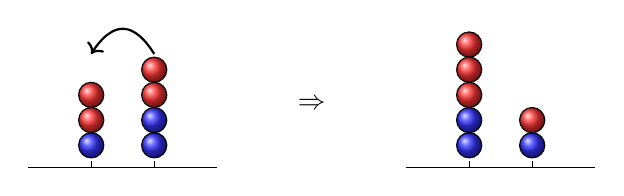
\begin{tikzpicture}[scale=0.8]
		\draw (-2,0)--(1,0);
		\foreach \x in {-1,0} 
		\draw  (\x,0) --+(0,0.1);
		%		\foreach \x/\y in {-1/2,0/3,1/4,2/5} 
		%		\node[below] at (\y,0) {$\x$};
		\foreach \x in {0,-1}
		\draw[shading=ball,ball color=blue!80] (\x,.35) circle (.2);
		\draw[shading=ball,ball color=blue!80] (0,.75) circle (.2);
		\draw[shading=ball,ball color=red!80] (0,1.15) circle (.2);
		\draw[shading=ball,ball color=red!80] (0,1.55) circle (.2);
		\draw[shading=ball,ball color=red!80] (-1,1.15) circle (.2);
		\draw[shading=ball,ball color=red!80] (-1,.75) circle (.2);
		\draw[<-,thick] (-1,1.8) parabola bend (-0.5,2.2) (0,1.8);
		\node at (2.5,1) {$\Rightarrow$};
		%		\node at (4.5,2.3) {$p$};
		%		\draw[->,thick] (4,1.7) parabola bend (3.5,2.1) (3,1.7);
		%		\node at (3.5,2.3) {$p^\prime$};
		%		\node [cross out,draw=red,thick]at (0.5,1.1) {};
		%		\node [cross out,draw=red,thick]at (-0.5,1.1) {};
		%		\draw[->,thick] (0,0.7) parabola bend (-0.5,1.1) (-1,.7);
		\draw (4,0)--(7,0);
		\foreach \x in {5,6} 
		\draw  (\x,0) --+(0,0.1);
		%		\foreach \x/\y in {-1/2,0/3,1/4,2/5} 
		%		\node[below] at (\y,0) {$\x$};
		\foreach \x in {5,6}
		\draw[shading=ball,ball color=blue!80] (\x,.35) circle (.2);
		\draw[shading=ball,ball color=red!80] (6,.75) circle (.2);
		\draw[shading=ball,ball color=red!80] (5,1.15) circle (.2);
		\draw[shading=ball,ball color=red!80] (5,1.55) circle (.2);
		\draw[shading=ball,ball color=red!80] (5,1.95) circle (.2);
		\draw[shading=ball,ball color=blue!80] (5,.75) circle (.2);
		%\draw[->,thick] (-1,1.8) parabola bend (-0.5,2.2) (0,1.8);
	\end{tikzpicture}
\end{table}	}
\end{frame}

\begin{frame}{Proof Outline}
	\small
\begin{table}
	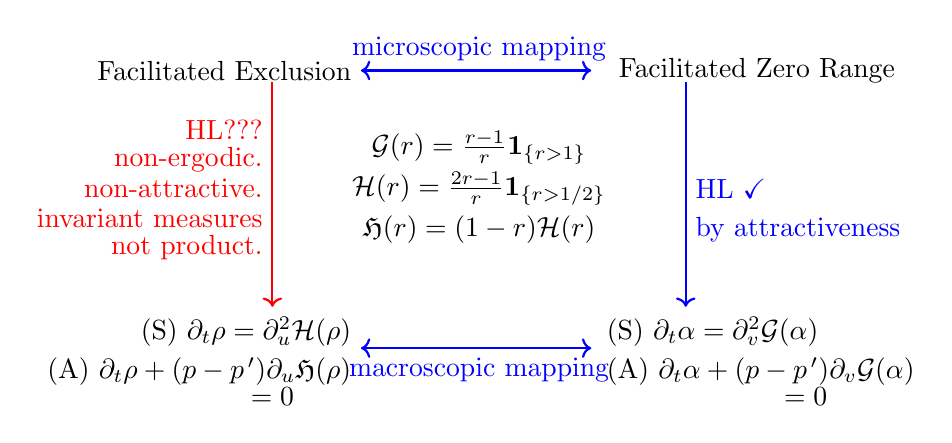
\begin{tikzpicture}[scale=0.75]
		\node [left] at (-2.5,2) {Facilitated Exclusion};
		\node [right] at (1.7,2) {Facilitated Zero Range};
		\node[below right]  at (1.5,-2) {(S) $\partial_t \alpha = \partial_v^2 \mathcal{G}(\alpha)$};
		\node[below right]  at (1.5,-2.7) {(A) $\partial_t \alpha + (p-p^{\,\prime})\partial_v \mathcal{G}(\alpha) $};
			\node[below right]  at (4.5,-3.2) {$=0 $};
		\node [below left] at (-2.5,-2) {(S) $\partial_{t} \rho=\partial_{u}^{2} \mathcal{H}(\rho)$};
		\node [below left] at (-2.5,-2.7) {(A) $\partial_{t} \rho+ (p-p^{\,\prime})\partial_{u} \mathfrak{H}(\rho)$};
			\node [below] at (-4,-3.2) {$=0$};
		\node at (-.5,0.7) {$\mathcal{G}(r)=\frac{r-1}{r} \mathbf{1}_{\{r>1\}}$};
		\node at (-.5,0) {$\mathcal{H}(r)=\frac{2r-1}{r} \mathbf{1}_{\{r>1/2\}}$};
		\node at (-.5,-0.7) {$\mathfrak{H}(r)=(1-r)\mathcal{H}(r)$};
		\draw[->,thick,color=blue] (3,1.8)--(3,-2);
		\draw[->,thick,color=red] (-4,1.8)--(-4,-2);
		\draw[<->,thick,color=blue] (-2.5,2)--(1.4,2);
		\draw[<->,thick,color=blue] (-2.5,-2.7)--(1.4,-2.7);
		\node[left] at (-4,1) {\color{red} HL???};
		\node[left] at (-4,.5) {\color{red} non-ergodic. };
		\node[left] at (-4,0) {\color{red} non-attractive.};
		\node[left] at (-4,-0.5) {\color{red} invariant measures};
		\node[left] at (-4,-1) {\color{red} not product.};
		\node[above] at (-0.5,2) {\color{blue} microscopic mapping};
		\node[right] at (3,0) {\color{blue} HL $\checkmark$};
		\node[right] at (3,-0.7) {\color{blue} by attractiveness};
		\node[below] at (-.5,-2.7) {\color{blue} macroscopic mapping};
	\end{tikzpicture}
\end{table}
\end{frame}

%\begin{frame}{Macroscopic Mapping}
%	\begin{itemize}
%		\item<1-> Exclusion $\eta_x$, $\rho(t,u)$; Zero range $\omega_y$, $\alpha (t,v)$.
%		\item<2-> Consider the process on $\mathbb{Z}$. For any $\varphi \in C_c (\mathbb{R})$,
%		\[\frac{1}{N}\sum_{x \in \mathbb{Z}} [1 - \eta_x (tN)] \varphi(x/N)  =  \frac{1}{N}\sum_{y \in \mathbb{Z}} \varphi (X_y (tN)/N).\]
%		\item<3-> Note that  \[X_y  = \sum_{y^\prime = 1}^y [X_{y^\prime} - X_{y^\prime-1}] + X_0 = \sum_{y^\prime = 1}^y [1+\omega_{y^\prime-1}] + X_0.\]
%		\item<4-> Let $\sigma_t = \lim_{N \rightarrow \infty} X_0 (tN)/N$,
%		\[\int (1-\rho(t,u)) \varphi (u) du = \int \varphi \Big( \int_0^v (1+\alpha(t,v^\prime) ) dv^\prime + \sigma_t\Big) dv\]
%	\end{itemize}
%\end{frame}

%\begin{frame}{Macroscopic Mapping}
%	
%\begin{itemize}
%	\item<1-> We already have
%		\[\int (1-\rho(t,u)) \varphi (u) du = \int \varphi \Big( \int_0^v (1+\alpha(t,v^\prime) ) dv^\prime + \sigma_t\Big) dv\]
%	\item<2-> Let
%	\[u(t,v) =  \int_0^v (1+\alpha(t,v^\prime) ) dv^\prime + \sigma_t\]
%	It has an inverse $v(t,u)$.
%	\item<3-> Then,
%	\[\int \varphi \Big( \int_0^v (1+\alpha(t,v^\prime) ) dv^\prime + \sigma_t\Big) dv = \int \varphi (u) [1+\alpha(t,v(t,u))]^{-1} du.\]
%	\item<4-> We finally have
%	\[\rho(t,u) = \frac{\alpha (t,v(t,u))}{1+\alpha (t,v(t,u))}.\]
%\end{itemize}
%\end{frame}

%\begin{frame}{Macroscopic Mapping}
%
%\begin{itemize}
%	\item<1-> Relation between $\alpha (t,v)$ and $\rho (t,u)$:
%		\[\rho(t,u) = \frac{\alpha (t,v(t,u))}{1+\alpha (t,v(t,u))},\]
%		\[u(t,v) =  \int_0^v (1+\alpha(t,v^\prime) ) dv^\prime + \sigma_t\].
%	\item<2-> Prove
%	\begin{align*}
%	&\rho(t,u) \text{\quad is solution of FEP}\\
%	\Leftrightarrow \quad  &\alpha (t,v) \text{\quad is solution of FZRP}.
%	\end{align*}
%\end{itemize}
%\end{frame}

%\begin{frame}{Macroscopic Mapping}
%	\begin{itemize}
%		\item<1->  Problem: the solutions to the Stefan problem and hyperbolic equation are not smooth.
%		\item<2-> For the Stefan problem 
%		\[\partial_{t} \rho=\partial_{u}^{2} \blue{\mathcal{H}} (\rho),\]  
%		we approximate the function $\mathcal{H}$ by some good $\mathcal{H}^\varepsilon$, 
%			\[\partial_{t} \rho^\varepsilon=\partial_{u}^{2} \blue{\mathcal{H}^\varepsilon} (\rho^\varepsilon).\] 
%		\item<3-> For the hyperbolic equation
%		\[\partial_{t} \rho+(2p-1)\partial_{u} \mathfrak{H}(\rho)=0,\]
%		we use viscous approximation method,
%		\[\partial_{t} \rho^\varepsilon+(2p-1)\partial_{u} \mathfrak{H}(\rho^\varepsilon)= \blue{\varepsilon \partial_{u}^2 \rho^\varepsilon}.\]
%	\end{itemize}
%\end{frame}

\begin{frame}{References}
\small
\begin{thebibliography}{9}
	\bibitem{1} Kipnis, C., \& Landim, C. (1998). {\it Scaling limits of interacting particle systems} (Vol. 320). Springer Science \& Business Media.
	\bibitem{2} Blondel, O., Erignoux, C., Sasada, M., \& Simon, M. (2020, February). Hydrodynamic limit for a facilitated exclusion process. {\it In Annales de l'Institut Henri Poincaré, Probabilités et Statistiques} (Vol. 56, No. 1, pp. 667-714). 
	\bibitem{3} Blondel, O., Erignoux, C., \& Simon, M. (2021). Stefan problem for a nonergodic facilitated exclusion process. {\it Probability and Mathematical Physics}, 2(1), 127-178.
	\bibitem{4} Erignoux, C., Simon, M., \& Zhao, L. (2022). Mapping hydrodynamics for the facilitated exclusion and zero-range processes. {\it arXiv preprint arXiv:2202.04469.}
\end{thebibliography}
\end{frame}

\logo{\includegraphics[scale=0.2]{school.png}}

\begin{frame}
	\begin{center}
		{\Huge Thanks!}
		
		\medspace
		
		{\it Email:} linjie.zhao@inria.fr
	\end{center}
\end{frame}

\end{document} 